\documentclass[conference]{IEEEtran}
\IEEEoverridecommandlockouts
\usepackage{cite}
\usepackage{amsmath,amssymb,amsfonts}
\usepackage{algorithmic}
\usepackage{graphicx}
\usepackage{textcomp}
\usepackage{xcolor}
\usepackage{bm}
\usepackage{here}
\usepackage{booktabs}
\def\BibTeX{{\rm B\kern-.05em{\sc i\kern-.025em b}\kern-.08em
    T\kern-.1667em\lower.7ex\hbox{E}\kern-.125emX}}
\begin{document}

\title{Phase Odometry: Trajectory Estimation \\ for Mobile Robots via Graph Optimization to Mitigate Error Accumulation by Complementing Wi-Wi Carrier Wave Phases and Odometry}

\author{
\IEEEauthorblockN{Takaaki Nara}
\IEEEauthorblockA{\textit{Graduate School of Information Sciences (GSIS)} \\
\textit{Tohoku University}\\
Sendai, Miyagi 980-8579, Japan \\
nara.takaaki@tr.is.tohoku.ac.jp}
~\\
\and
\IEEEauthorblockN{Yoshito Okada}
\IEEEauthorblockA{\textit{Tough Cyberphysical AI Research Center(TCPAI)} \\
\textit{Tohoku University}\\
Sendai, Miyagi 980-8579, Japan \\
okada@tr.is.tohoku.ac.jp}
~\\
\and
\IEEEauthorblockN{Shotaro Kojima}
\IEEEauthorblockA{\textit{TCPAI} \\
\textit{Tohoku University}\\
Sendai, Miyagi 980-8579, Japan \\
kojima@tr.is.tohoku.ac.jp}
~\\
\and
\IEEEauthorblockN{Yoshiki Yokota}
\IEEEauthorblockA{\textit{GSIS} \\
\textit{Tohoku University}\\
Sendai, Miyagi 980-8579, Japan \\
yokota.yoshiki@tr.is.tohoku.ac.jp}
~\\
\and
\IEEEauthorblockN{Ranulfo Bezerra}
\IEEEauthorblockA{\textit{TCPAI} \\
\textit{Tohoku University}\\
Sendai, Miyagi 980-8579, Japan \\
bezerra.ranulfo@tr.is.tohoku.ac.jp}
\and
\IEEEauthorblockN{Kazunori Ohno}
\IEEEauthorblockA{\textit{TCPAI/GSIS} \\
\textit{Tohoku University}\\
Sendai, Miyagi 980-8579, Japan \\
kazunori@tr.is.tohoku.ac.jp}
\and
\IEEEauthorblockN{Nobuyasu Shiga}
\IEEEauthorblockA{\textit{National Institute of Information and Communications Technology (NICT)} \\
Koganei, Tokyo 184-8795, Japan \\
shiga@nict.go.jp}
\and
\IEEEauthorblockN{Satoshi Yasuda}
\IEEEauthorblockA{\textit{NICT} \\
Koganei, Tokyo 184-8795, Japan \\
sayasuda@nict.go.jp}
\and
\IEEEauthorblockN{Kenichi Takizawa}
\IEEEauthorblockA{\textit{NICT} \\
Koganei, Tokyo 184-8795, Japan \\
takizawa@nict.go.jp}
~\\
\and
\IEEEauthorblockN{Satoshi Tadokoro}
\IEEEauthorblockA{\textit{TCPAI} \\
\textit{Tohoku University}\\
Sendai, Miyagi 980-8579, Japan \\
tadokoro@tr.is.tohoku.ac.jp}
}

\maketitle


\begin{abstract}
We present a graph-optimization approach that jointly estimates a mobile robot trajectory and the unknown positions of wireless fixed bases by fusing time-differenced carrier phases measured with Wi-Wi and wheel odometry. Robot poses and base locations are modeled as nodes; edges encode odometry increments and carrier-phase differences, avoiding the 2π ambiguity while exploiting the high precision of phase. Minimizing the weighted sum of edge residuals suppresses odometry drift and yields consistent estimates. 
Indoor experiments over a 120-m trajectory demonstrate sub-meter robot localization and some base positions where estimated with an error as low as 0.11 m, indicating accurate localization in GNSS-denied environments.
\end{abstract}

\begin{IEEEkeywords}
Localization, mobile robot, wireless two-way interferometry (Wi-Wi)
\end{IEEEkeywords}

\section{Introduction}


Localization techniques that leverage radio carrier-phase measurements have attracted attention in domains 
\begin{figure}[H]
    \centering
    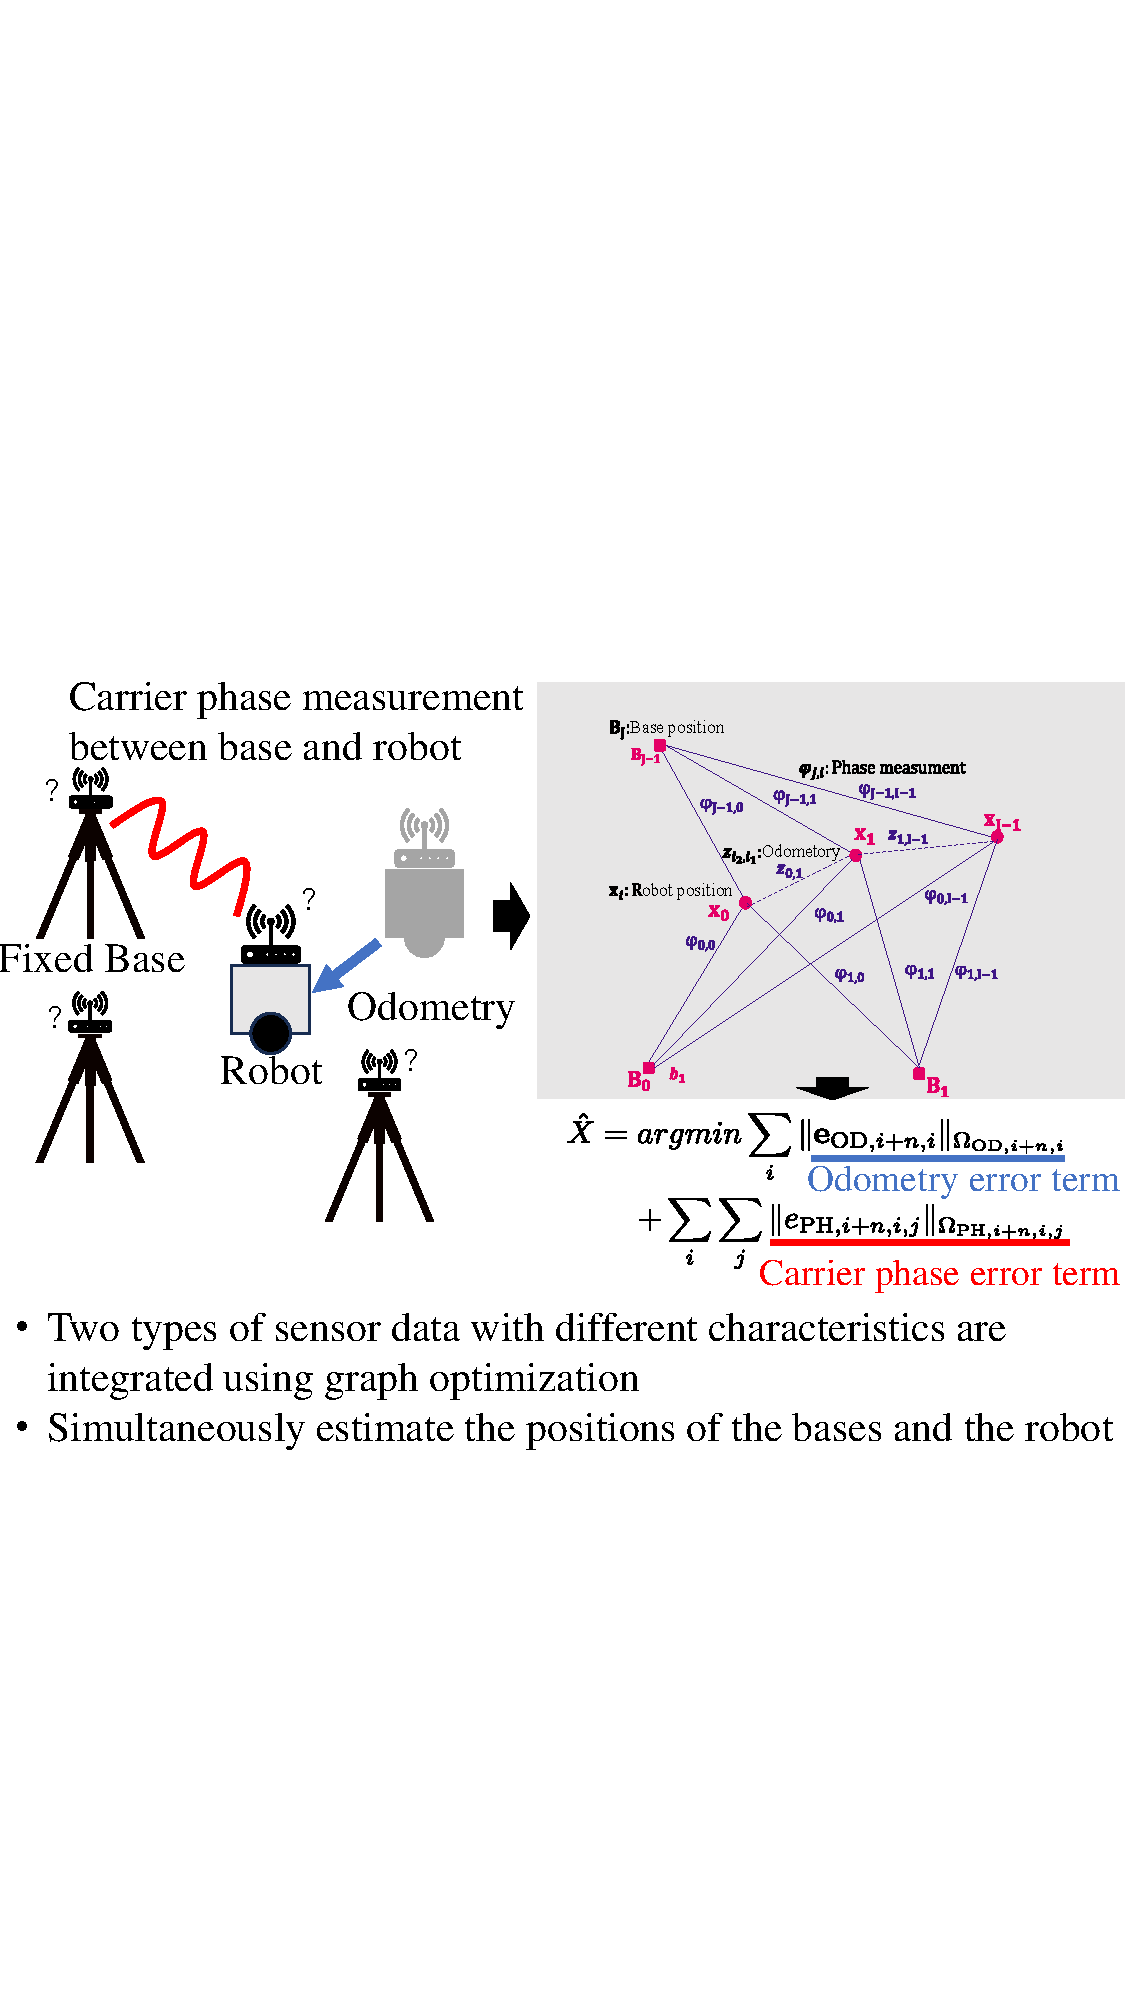
\includegraphics[width=0.99\linewidth]{figures/Fig1.pdf}
    \caption{The simultaneous estimation of the robot's position and the fixed bases' position is based on graph optimization using carrier phase and odometry measurements.}
    \label{fig:fig1}
\end{figure}
such as autonomous driving because they provide higher measurement accuracy than approaches based on received signal strength or code-based pseudoranges~\cite{gnss_autonomou_vehicles}.
Real-Time Kinematic Global Navigation Satellite System (RTK-GNSS)~\cite{RTK-GNSS} is a representative carrier-phase-based positioning method.
RTK-GNSS can estimate the position of a receiving antenna with an accuracy of several centimeters and has been applied in drones~\cite{RTK-M300}, agriculture~\cite{RTK-Agriculture}, construction~\cite{six-dump}, and many other fields.
However, GNSS requires line of sight to satellites and suffers from accuracy degradation caused by natural phenomena such as ionospheric conditions and geomagnetic disturbances~\cite{gnss_error}.

As an alternative to RTK-GNSS, we study a localization method based on carrier-phase measurements supported by wireless two-way interferometry (Wi-Wi)~\cite{Shiga2017,Yasuda2019}, a precise wireless time-synchronization technology.
In carrier-phase measurements, the drift of internal clocks among radio terminals directly affects ranging.
Conventional solutions either rely on highly accurate but expensive atomic clocks, as with GNSS, or on wired connections with limited deployment flexibility, making it difficult to adopt carrier-phase measurements on mobile robots.
Wi-Wi synchronizes the clocks of communication devices at the sub-nanosecond level through a bidirectional wireless protocol implemented with commercial-off-the-shelf radios.
As illustrated in Fig.~\ref{fig:fig1}, we place Wi-Wi terminals both on the robot and in the environment and exploit the precise phase information measured using Wi-Wi's accurate time synchronization to achieve higher localization accuracy than existing approaches.

Nevertheless, two challenges must be addressed to realize localization with Wi-Wi.
First, carrier-phase measurements exhibit a $2\pi$ ambiguity: the phase value repeats with a period of $2\pi$, meaning the absolute distance between antennas cannot be directly retrieved from a single measurement.
Therefore, using the raw phase measurements alone does not yield an accurate position estimate, and additional processing is required.
Second, we assume that users can freely place the fixed bases.
The relative arrangement of the bases is initially unknown, yet we must estimate both the base configuration and the robot trajectory solely from ambiguous phase measurements.

To overcome these challenges, we propose a graph-optimization-based localization method that fuses differences of carrier-phase measurements taken at different time steps with wheel odometry derived from the rotation of the robot's tires.
The key idea is to build a graph whose edges incorporate both the highly accurate but ambiguous carrier-phase differences and the less accurate but ambiguity-free motion increments obtained from odometry.
By complementing each modality, the method suppresses the accumulation of errors.
Treating the fixed bases as unknown parameters within the graph further enables simultaneous estimation of the base positions and the robot trajectory even when prior knowledge about the deployment is limited.

This paper analyzes the characteristics of the proposed method through simulation and evaluates its accuracy in real-world indoor experiments.
The results show that the proposed method estimates the robot's position with sub-meter accuracy in indoor environments where radio-based localization is challenging, while the fixed-base positions are recovered with errors as small as 0.11~m.

\section{Related Work}
Wireless two-way interferometry (Wi-Wi) synchronizes clocks between radio terminals by bidirectionally measuring carrier phases and compensating for clock offsets.
The Wi-Wi terminals used in this study employ the 920~MHz band, achieving 30~ns timing synchronization accuracy and 20~ps phase (jitter) synchronization accuracy~\cite{ouchi2024evaluation}.
Existing Wi-Wi research includes delay-constrained wireless networking enabled by precise synchronization~\cite{Yamasaki2021} and estimation of atmospheric water vapor based on propagation characteristics~\cite{Yasuda2019}.
Building on this line of research, we propose a graph-optimization-based localization method that places Wi-Wi terminals on both the mobile robot and the environment and utilizes carrier-phase measurements between the robot and fixed bases.

Graph-based optimization is a powerful approach to minimizing motion and pose errors in robot trajectory estimation, and extensive research has explored simultaneous localization and mapping (SLAM) using cameras, LiDAR, and odometry~\cite{grisetti2010tutorial,graph_slam_urban_mapping,graph_slam_2012}.

Carrier-phase-based localization methods that exploit time-differenced carrier phase (TDCP) measurements, which subtract GNSS carrier phases across time, have also been investigated~\cite{TDCP2008,TDCP2022}.
TDCP eliminates the ambiguity inherent in carrier phases and delivers high accuracy even in multipath environments.
GNSS odometry, which combines TDCP with graph-based optimization to estimate trajectories using a single GNSS receiver, has been proposed~\cite{suzuki2022gnss}.
These GNSS-based approaches provide excellent accuracy when satellite signals are available, but they are difficult to deploy indoors, where signals are blocked.
In contrast, our goal is to localize by deploying wireless fixed bases even in environments where GNSS cannot be used, enabling the simultaneous estimation of both base locations and the robot trajectory.

\section{Trajectory Estimation via Graph Optimization Combining Odometry and Carrier Phase Differences}
\subsection{Overview}
In the proposed system, multiple Wi-Wi terminals installed in the environment act as fixed bases, and the mobile robot is equipped with a Wi-Wi terminal capable of communicating with the bases as well as an odometry sensor that measures its motion.
The bases are assumed to be multiple, and their relative positions are unknown.
Phase measurements can be obtained from all bases within communication range, and each measurement can be associated with the corresponding base.
The robot records odometry and carrier-phase measurements while moving.
Because odometry typically updates faster, we treat the robot pose at the instant of each carrier-phase measurement as the odometry pose, effectively assuming synchronized measurement timings.

\subsection{Graph Structure and Notation}
The graph to be optimized is illustrated in Fig.~\ref{fig:graph_structure}.
The graph contains $J$ fixed-base nodes ($\mathbf{B}_j$) and $I$ robot nodes ($\mathbf{x}_i$), where $i$ indexes the robot poses at which carrier-phase measurements are obtained.
Edges between robot nodes encode odometry measurements $\mathbf{z}$, while edges between robot nodes and fixed-base nodes encode carrier-phase measurements $\phi$.

\begin{figure}[tb]
    \centering
    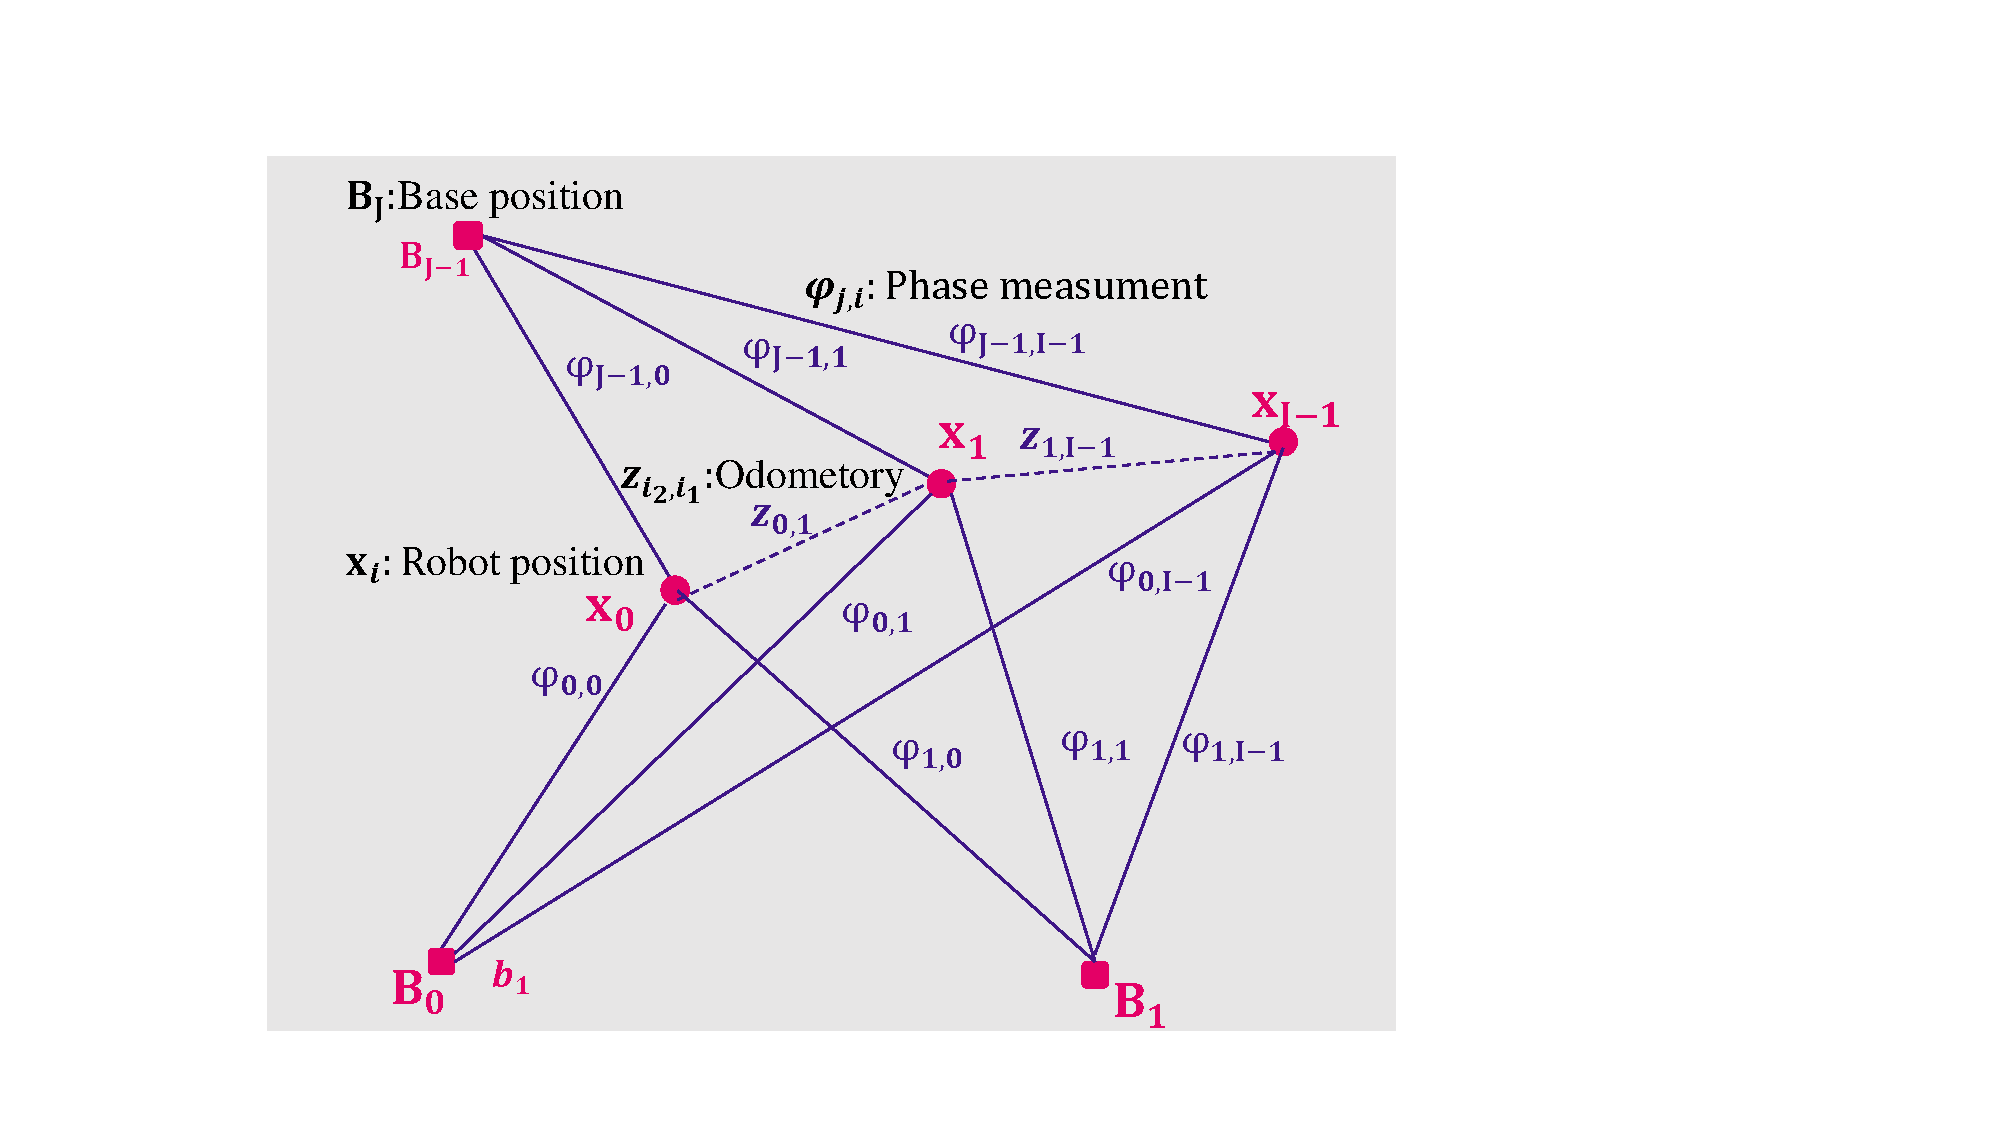
\includegraphics[width=0.95\linewidth]{figures/graph.pdf}
    \caption{Graph structure to be optimized in the proposed method.}
    \label{fig:graph_structure}
\end{figure}

The set of state variables in the proposed method is defined as
\begin{equation}
    \mathbf{X} = \left[\mathbf{\hat{x}}_0\, \mathbf{\hat{x}}_1\, \mathbf{\hat{x}}_2\, \cdots \mathbf{\hat{x}}_{I-1}\, \mathbf{\hat{B}}_0\, \mathbf{\hat{B}}_1\, \cdots \mathbf{\hat{B}}_{J-1}\, \mathbf{\hat{H}}\right].
\end{equation}
Here $\mathbf{\hat{H}}$ is the transformation matrix from the robot's odometry frame to the estimation frame.
The state variables of each node are given by
\begin{equation}
   \mathbf{\hat{x}}_i = \left[\mathbf{p}_i\, \theta_{i}\right], \quad
   \mathbf{\hat{B}}_j = \left[\mathbf{p}'_j\right],
\end{equation}
where $\mathbf{p}$ denotes the position $(x,y)$ of each node in the 2-D estimation frame and $\theta_i$ is the yaw angle in the $xy$-plane.
The bases are assumed to have isotropic antennas, so orientation information is not included.

Graph-based pose estimation suffers from a gauge freedom: applying a common translation and rotation to all nodes leaves the cost unchanged, preventing a unique solution.
We remove this degree of freedom by fixing $\mathbf{B}_0$ at the origin and aligning the $x$-axis with the direction from $\mathbf{B}_0$ to $\mathbf{B}_1$.
Accordingly, $\mathbf{B}_0$ is set to $(0,0)$ and $\mathbf{B}_1$ lies on the $x$-axis as $(p'_{x,1}, 0)$ during optimization.

\subsection{Objective Function}
The objective function minimized by the optimization is composed of error terms derived from odometry measurements, $\mathbf{e}_{\mathrm{OD}}$, and carrier-phase measurements, $e_{\mathrm{PH}}$, weighted by information matrices $\Omega$ that encode the confidence of each measurement:
\begin{align}
    \hat{\mathbf{X}} = \arg\min_{\mathbf{X}} &\sum_{i}\|\mathbf{e}_{\mathrm{OD},i+n,i}\|_{\Omega_{\mathrm{OD},i+n,i}} \\
    +& \sum_{i}\sum_{j}\|e_{\mathrm{PH},i+n,i,j}\|_{\Omega_{\mathrm{PH},i+n,i,j}}.
\end{align}

\subsection{Odometry Error Term}
We adopt the odometry error formulation used in conventional graph SLAM~\cite{graph_slam}.
% The robot state in the odometry frame is defined as
% \begin{equation}
%     \mathbf{x}_i = [\mathbf{p}_i\, \theta_i].
% \end{equation}
The odometry measurement $\mathbf{z}_{i+n,i}$ relating states $\mathbf{x}_i$ and $\mathbf{x}_{i+n}$ is given by
\begin{equation}
    \mathbf{z}_{i+n,i} = \mathbf{h}(\mathbf{x}_{i+n}, \mathbf{x}_{i}) + \mathbf{w}_{i+n,i},
\end{equation}
where $\mathbf{h}(\cdot)$ is the sensor model and $\mathbf{w}_{i+n,i}$ denotes measurement noise.
The corresponding error function between the estimates $\mathbf{\hat{x}}_i$ and $\mathbf{\hat{x}}_{i+n}$ is
\begin{equation}
    \mathbf{e}_{\mathrm{OD},i+n,i} = \left(\mathbf{\hat{x}}_{i+n} - \mathbf{\hat{x}}_{i}\right) - \mathbf{\hat{H}}\mathbf{z}_{i+n,i},
\end{equation}
% with the weighted squared error
% \begin{equation}
%     \|\mathbf{e}_{\mathrm{OD},i+n,i}\|_{\Omega_{\mathrm{OD},i+n,i}} = \mathbf{e}_{\mathrm{OD},i+n,i}\, \Omega_{\mathrm{OD},i+n,i}\, \mathbf{e}_{\mathrm{OD},i+n,i}.
% \end{equation}

\subsection{Carrier Phase Error Term}
The carrier-phase measurement obtained from Wi-Wi is modeled as~\cite{Peng2017}
\begin{equation}
     \phi_{i,j} = \phi_{D,i,j} + \frac{1}{2}\pi K_i + w^{\phi}_{i,j},
\end{equation}
where $\phi_{D,i,j}$ represents the phase change accumulated during propagation between antennas, $K_i$ is the the integer bias used to unwrap the phase every half wavelength from the start of measurement, and $w^{\phi}_{i,j}$ denotes measurement noise.
Although Wi-Wi resolves the ambiguity by continuously unwrapping the phase from the beginning of the experiment, reflected multipath signals can cause incorrect integer-bias updates, leading to accumulated errors.
Therefore, instead of linking a robot node to a base node using a single phase observation, we define error functions using the difference between phase measurements at poses $i$ and $i+n$.
If the phase measurements are error free, the difference corresponds to the difference in distances between the robot poses and the base.
Letting $\lambda$ denote the wavelength, the error term is defined as
\begin{equation}
    e_{\mathrm{PH},i+n,i,j} = \left(\|\mathbf{\hat{p}}_{i+n} - \mathbf{\hat{B}}_j\| - \|\mathbf{\hat{p}}_{i} - \mathbf{\hat{B}}_j\|\right) - \lambda (\phi_{i+n,j} - \phi_{i,j}),
\end{equation}
% with the weighted squared error
% \begin{equation}
%     \|e_{\mathrm{PH},i+n,i,j}\|_{\Omega_{\mathrm{PH},i+n,i,j}} = e_{\mathrm{PH},i+n,i,j} \, \Omega_{\mathrm{PH},i+n,i,j} \, e_{\mathrm{PH},i+n,i,j}.
% \end{equation}

% \section{Simulation Experiments}
% We evaluated the effectiveness of combining the odometry and carrier-phase error terms in a simulation environment.
% Three conditions were compared: using odometry only, using phase information only, and the proposed fusion of phase and odometry.
% The simulation was implemented on ROS~1 (Noetic), and the proposed method was realized as a ROS node using the Ceres Solver~\cite{ceres-solver} for nonlinear optimization.
% The specifications of the PC and solver parameters are summarized in Table~\ref{tab:simpc}.

% % \input{tables/simpc}

% \subsection{Experimental Setup}
% The simulation models a 10~m\,$\times$\,10~m indoor area where both the robot and four fixed bases lie on a two-dimensional plane.
% We assume that the Wi-Wi terminals on the bases and the robot share the same height, so altitude is not estimated.
% The bases are placed at the four corners of the area.
% The robot starts at $(x,y)=(1,1)$~m, moves around the perimeter, and then heads toward the center at $(5,5)$~m.
% Carrier-phase and odometry measurements are obtained at 20~Hz.
% Gaussian noise with zero mean and 0.01~m standard deviation is added to the phase measurements.
% For the odometry, translational noise follows a zero-mean Gaussian distribution with 0.1~m standard deviation per meter of travel, and rotational noise has zero mean and 0.1~rad standard deviation.
% Optimization is executed online every time a new measurement arrives.

% We compare three conditions: odometry only, phase only, and the proposed fusion.
% The base positions are estimated in the phase-only and proposed conditions.
% The initial values used for the bases are listed in Table~\ref{tab:initial}, offset by approximately one meter from the ground truth.
% The odometry-only condition does not perform optimization; it directly integrates the odometry measurements.
% The phase-only condition initializes the robot nodes with the previous optimization result, whereas the proposed method initializes them with the current odometry measurements.

% \begin{table}
%     \centering
%     \caption{Initial values used for the estimation of fixed bases.}
%     \begin{tabular}{|c|c|c|c|}
%     \hline
%         & $\mathbf{B}_1$ & $\mathbf{B}_2$ & $\mathbf{B}_3$ \\ \hline
%        True value [m] &(10,0)  &(10,10) &(0,10) \\ \hline
%        Initial value [m] &(9,0)  &(11,11) &(0,11) \\ \hline
%     \end{tabular}
%     \label{tab:initial}
% \end{table}

% \subsection{Results}
% Figures~\ref{fig:trajectory_sim}(a)--(c) show the estimated robot trajectory and base positions under each condition, and Fig.~\ref{fig:trajectory_sim}(d) plots the Euclidean trajectory error against the travel distance.
% With odometry alone, the estimation error accumulates over time.
% Phase-only estimation largely follows the path but occasionally deviates significantly.
% In the proposed method, the trajectory converges to the true path near the corner at $(9,9)$~m and subsequently maintains approximately 0.1~m error.

% Figure~\ref{fig:trajectory_sim}(e) reports the estimation error for base $\mathbf{B}_2$, representative of the largest error among the bases.
% Table~\ref{tab:base_error} summarizes the final estimation errors for all bases using the measurements up to the end of the trajectory.
% \begin{table}
%     \centering
%     \caption{Position estimation accuracy for each fixed base in the simulation.}
%     \begin{tabular}{|c|c|c|c|}
%     \hline
%     & $\mathbf{B}_1$ & $\mathbf{B}_2$ & $\mathbf{B}_3$ \\
%     \hline
%     phase & 0.025~m & 0.208~m & 0.214~m \\
%     \hline
%     phase+odom & 0.043~m & 0.168~m & 0.083~m \\
%     \hline
%     \end{tabular}
%     \label{tab:base_error}
% \end{table}

% The proposed method converges around a travel distance of 20~m, whereas the phase-only condition occasionally exhibits error spikes even when convergence is observed.

% \subsection{Discussion}
% The simulation results demonstrate that the proposed method can estimate both the base arrangement and the robot trajectory online even when the base positions are unknown beforehand.
% Because the graph grows as new measurements are appended, data collection must continue until the estimation converges.
% However, an excessively large graph can increase computation time, which is problematic for online estimation that must finish within fixed time intervals.
% Future work includes resampling strategies and other mechanisms to bound the computational cost.

\section{Indoor Experiments with a Real Robot}
The proposed method targets indoor environments where GNSS is unavailable, so we evaluated it using a real system indoors.
Experiments were conducted in a laboratory room measuring 7.4~m by 11.2~m, with desks and shelves along the walls.

\subsection{Experimental System}
The experimental system is implemented on ROS~1 (Noetic), as in the simulation.
Wi-Wi terminals provide phase information for all terminal pairs through a single unit connected to a PC via USB-Serial.
One of the bases is connected to the PC to record the phase data.
Robot control commands and odometry are exchanged over Wi-Fi, and the ground-truth robot pose and base positions are recorded at 120~Hz using a motion-capture system.

The robot and bases used in the experiment are shown in Fig.~\ref{fig:robot}.
The robot is a custom platform for Wi-Wi carrier-phase measurements built on a mecanum-wheeled base with a transceiver antenna mounted at a height of 1.3~m.
The robot is manually teleoperated, with velocity commands sent from the experiment PC to the onboard controller over Wi-Fi.
Odometry is computed from wheel rotations by the onboard controller and transmitted to the PC.

\begin{figure}
    \centering
    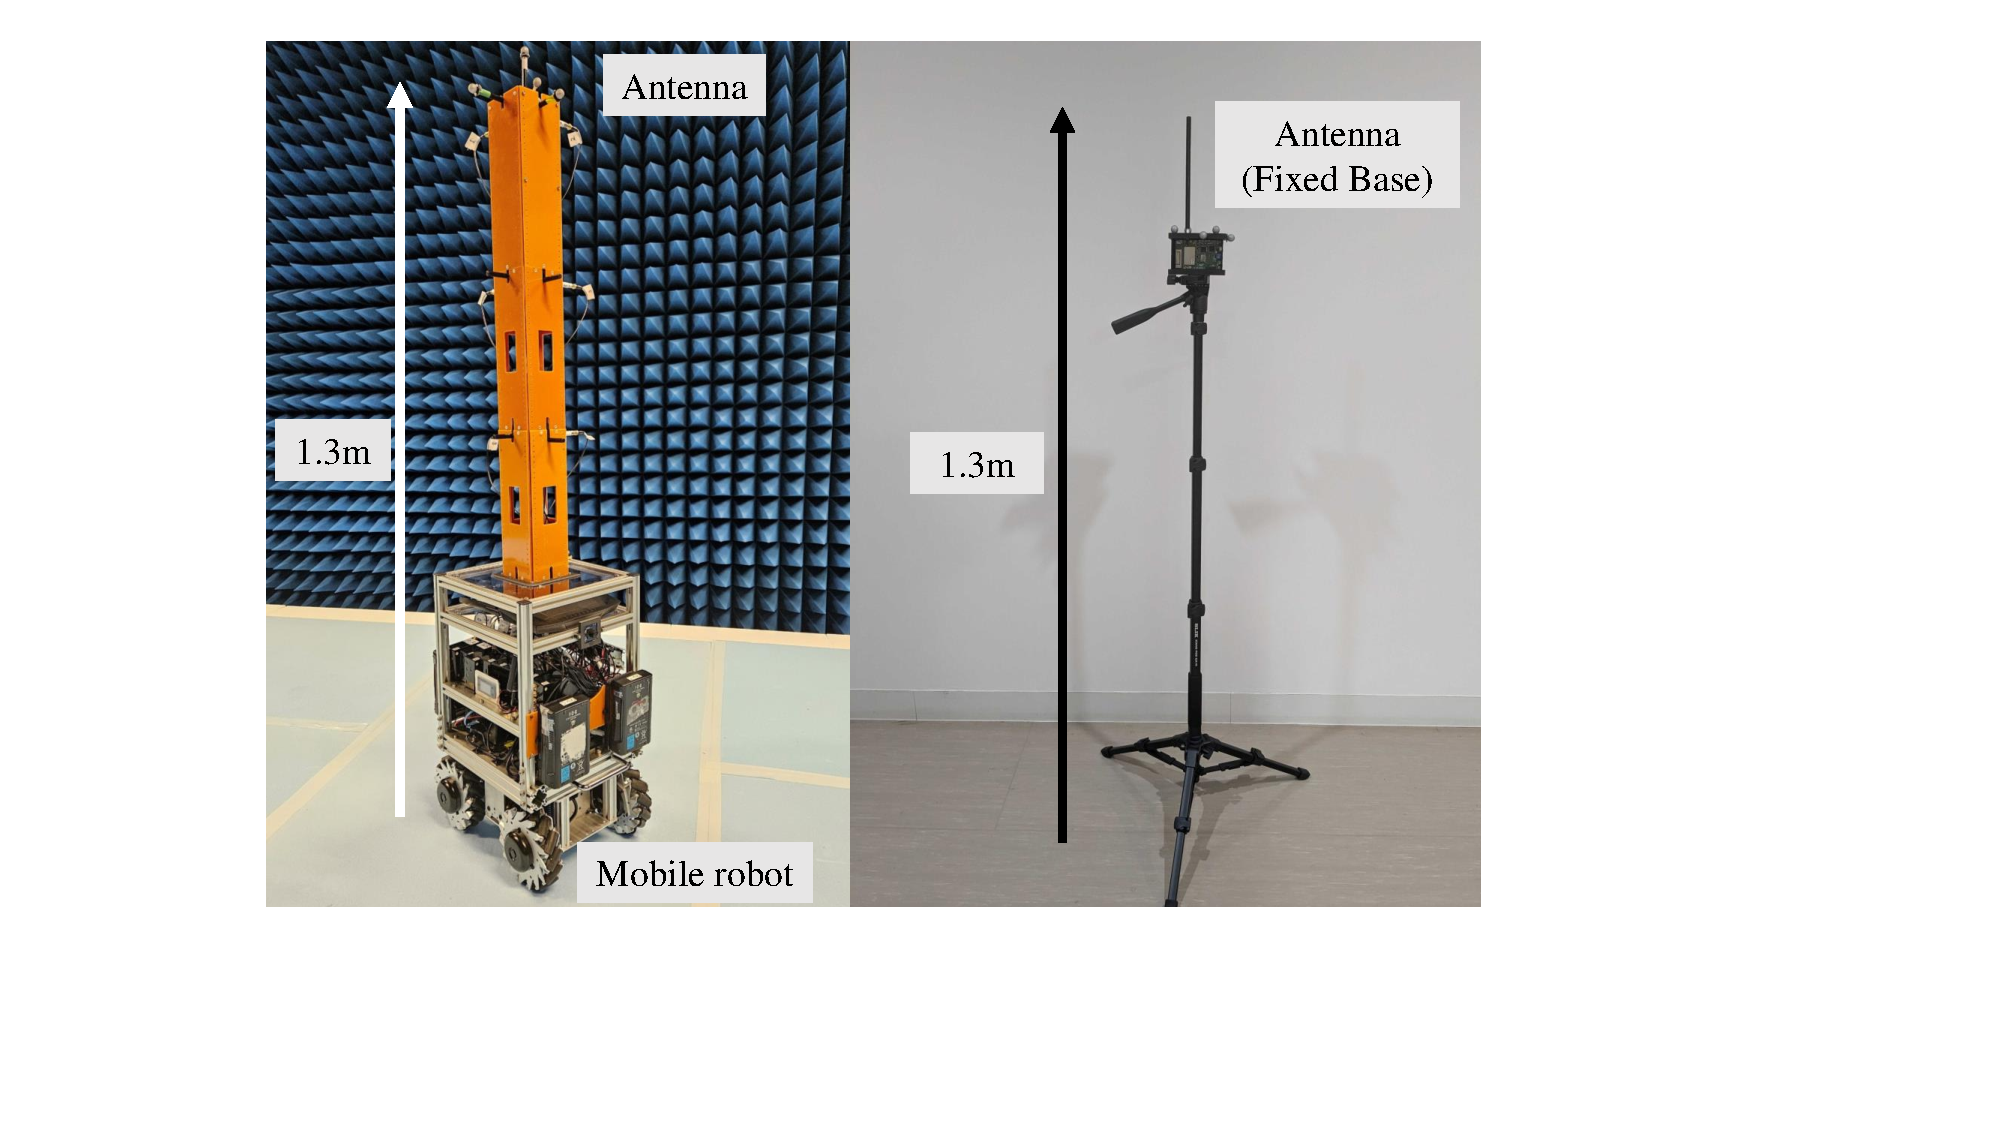
\includegraphics[width=0.95\linewidth]{figures/robot}
    \caption{Appearance of the robot and fixed base used in the experiment.}
    \label{fig:robot}
\end{figure}

\subsection{Experimental Conditions}
As in the simulation, we estimate the two-dimensional positions of the robot and four bases.
The true base positions and the initial values used for optimization are listed in Table~\ref{tab:initial_real}.

The robot is teleoperated to follow an arbitrary path, traveling approximately 120~m over 400~s.
Although optimization is triggered online whenever new measurements arrive, the computation currently exceeds the 20~Hz measurement rate of Wi-Wi, so the system does not yet satisfy real-time constraints.

\begin{table}
    \centering
    \caption{Initial values used to estimate fixed bases in the experiment.}
    \begin{tabular}{ccccc}
    \toprule
        &$\mathbf{B}_0$ & $\mathbf{B}_1$ & $\mathbf{B}_2$ & $\mathbf{B}_3$ \\
    \midrule
       True [m]  &$(0,0)$&$(2.79,0)$  &$(3.58,3.67)$ &$(-0.09,3.67)$ \\
       Initial [m] &$(-,-)$&$(3.79,-)$  &$(3.58,4.67)$ &$(0.91,4.67)$ \\
    \bottomrule
    \end{tabular}
    \label{tab:initial_real}
\end{table}

\subsection{Results}
Figure~\ref{fig:error_real} shows the localization error of the proposed method computed against the motion-capture ground truth.
While the odometry error accumulates with travel distance, the proposed method maintains errors below roughly 1~m.

Table~\ref{tab:base_error_real} lists the estimated base positions at the end of the trajectory.
Base~1 is recovered with 0.11~m error, whereas bases~2 and 3 have errors of approximately 1.7~m and 0.787~m, respectively.
Figure~\ref{fig:error_base} plots the error evolution for bases~1 and 2, the smallest and largest errors among the bases, showing that the error for base~2 converges around 1.7~m.

\begin{figure}
    \centering
    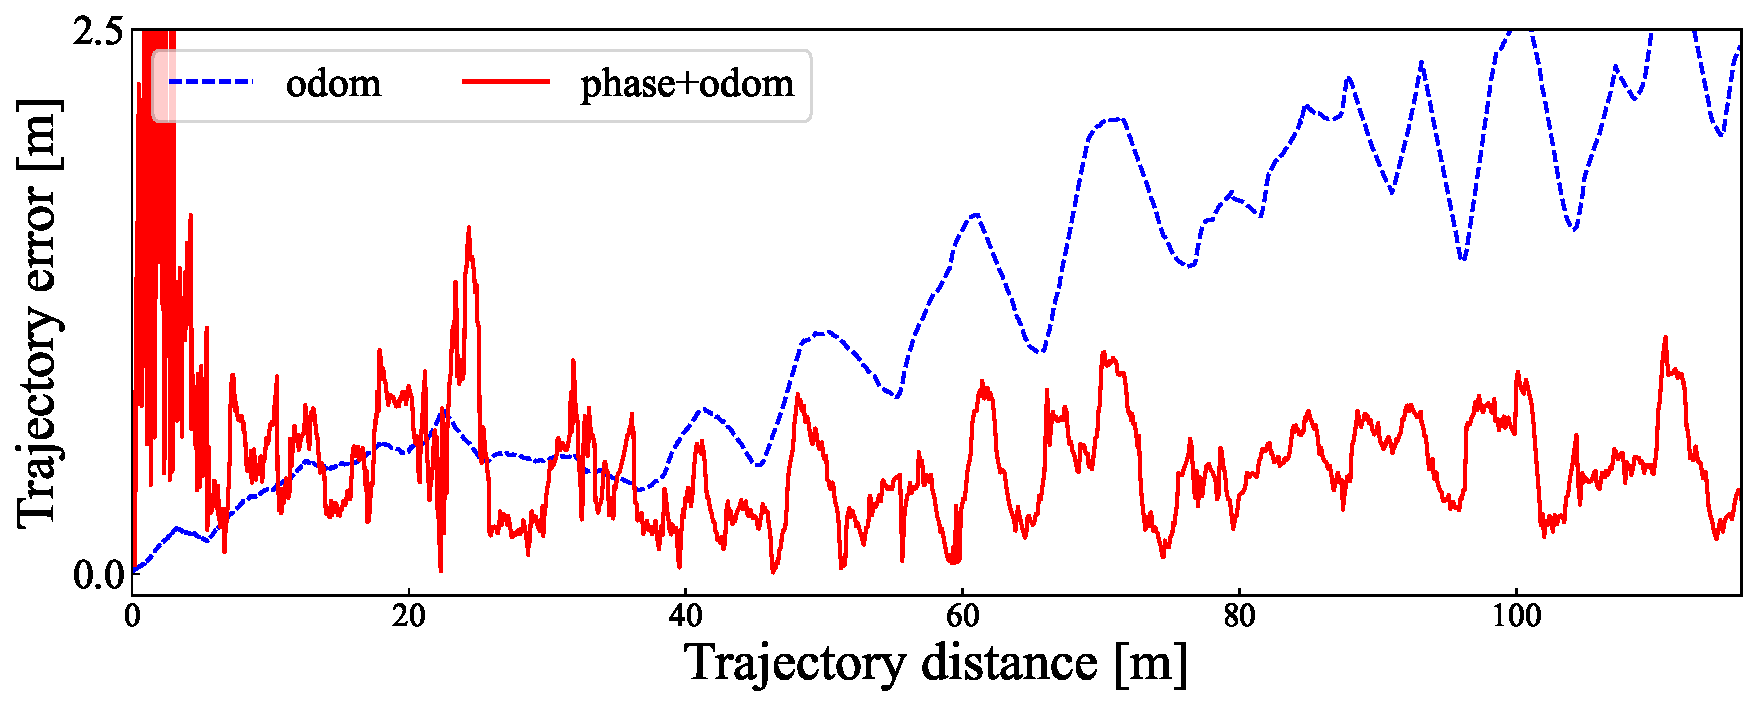
\includegraphics[width=0.95\linewidth]{project/figures/icara_1018_resutl_2_online_rover_position_error_comparison.pdf}
    \caption{Position estimation errors of the robot relative to the trajectory distance.}
    \label{fig:error_real}
\end{figure}

\begin{figure}
    \centering
    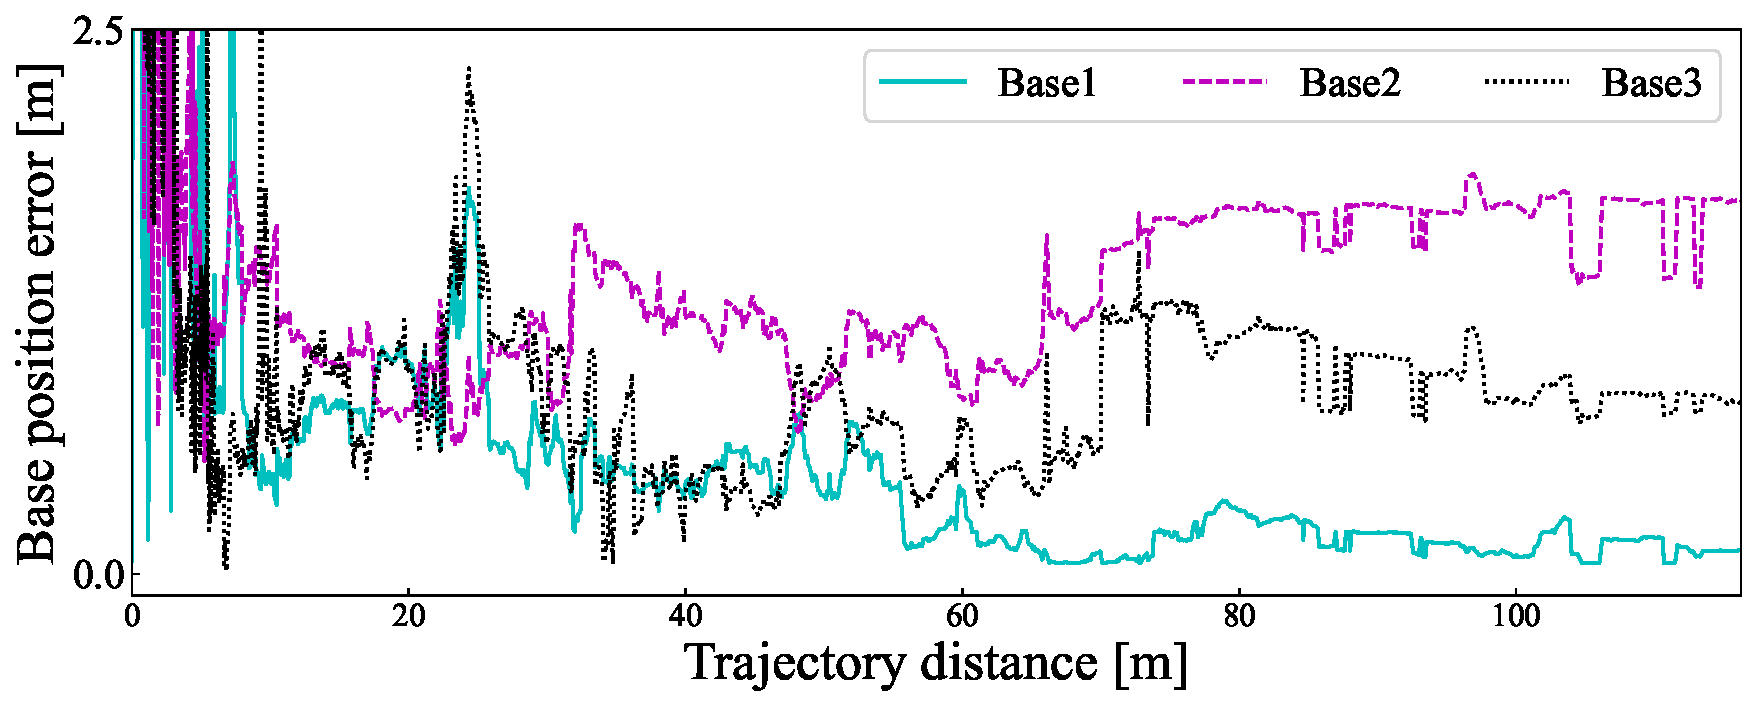
\includegraphics[width=0.95\linewidth]{project/figures/icara_1018_resutl_2_online_base_position_error_comparison.pdf}
    \caption{Position estimation errors of the bases relative to the trajectory distance.}
    \label{fig:error_base}
\end{figure}

\begin{table}
    \centering
    \caption{Position estimation accuracy for each fixed base in the real-world experiment.}
    \begin{tabular}{ccccc}
    \toprule
    &$\mathbf{B}_0$& $\mathbf{B}_1$ & $\mathbf{B}_2$ & $\mathbf{B}_3$ \\
    \midrule
    phase+odom &-&0.11~m & 1.711~m & 0.787~m \\
    \bottomrule
    \end{tabular}
    \label{tab:base_error_real}
\end{table}

These results show that simply deploying wireless bases indoors, where GNSS is unavailable, allows the proposed method to estimate the robot position with sub-meter accuracy and the base positions with errors as low as 0.11~m.

\subsection{Discussion}
We analyze the estimator's behavior from the perspective of Wi-Wi carrier-phase measurement accuracy.
Figure~\ref{fig:vicon_vs_wiwi} compares the phase-difference reference derived from motion capture with the Wi-Wi measurements for the base that yielded the smallest error (base~1).
All bases exhibited similar trends.
Table~\ref{tab:vicon_vs_wiwi} summarizes the root-mean-square error (RMSE) between the reference and measured phase differences, showing an average precision of approximately 0.03~m.
However, Fig.~\ref{fig:vicon_vs_wiwi} reveals spike-like outliers, likely caused by reflected multipath signals.
Although the optimization can still achieve 0.1~m accuracy in some instances despite these spikes, they also explain the 1.7~m error observed for base~2.
Future work includes rejecting measurements affected by strong reflections to further improve accuracy.

\begin{figure}
    \centering
    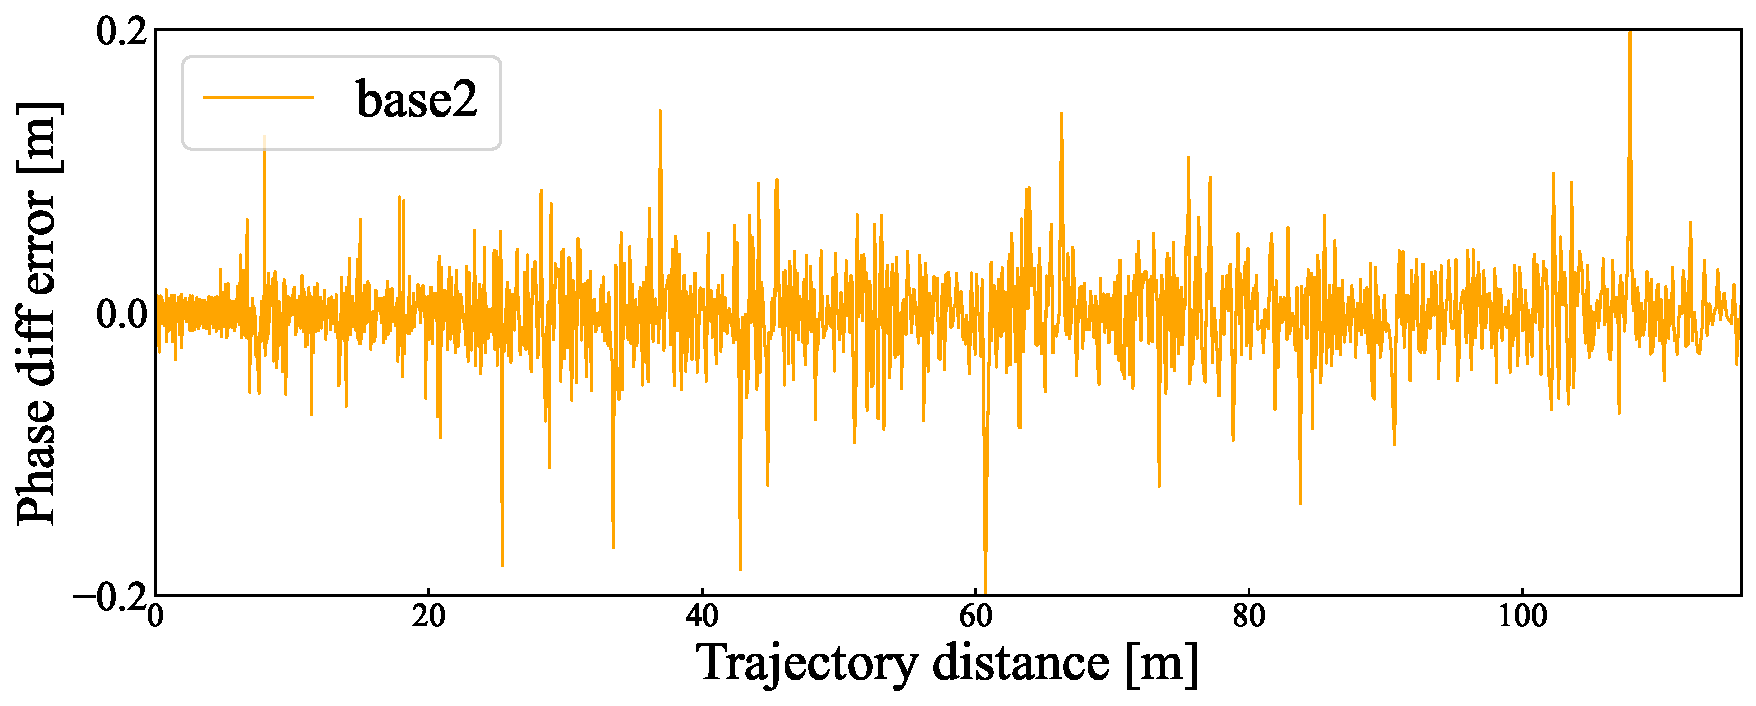
\includegraphics[width=0.99\linewidth]{project/figures/icara_1018_resutl_2_online_distance_pdm2_differences.pdf}
    \caption{Difference between the reference phase differences calculated from motion capture and the phase differences measured by Wi-Wi (base~1).}
    \label{fig:vicon_vs_wiwi}
\end{figure}

\begin{table}[tb]
    \centering
    \caption{RMSE between the reference and measured values of phase differences.}
    \begin{tabular}{ccccc}
    \toprule
         & $\mathrm{B}_0$ & $\mathrm{B}_1$ & $\mathrm{B}_2$ & $\mathrm{B}_3$ \\
    \midrule
     RMSE [m] & 0.035 & 0.027 & 0.029 & 0.025 \\
     \bottomrule
    \end{tabular}
    \label{tab:vicon_vs_wiwi}
\end{table}

\section{Conclusion}
We proposed a graph-optimization method that combines carrier-phase differences and odometry to simultaneously estimate the trajectory of a mobile robot and the positions of wireless fixed bases.
Simulation experiments confirmed that incorporating phase differences between consecutive odometry poses suppresses the accumulation of odometry errors and improves estimation accuracy.
Real-world experiments demonstrated that the method achieves sub-meter accuracy for robot localization and 0.11~m accuracy for base localization in indoor environments where GNSS cannot be used.
Future work includes mitigating multipath-induced outliers and reducing computation time toward real-time operation.

\section*{Acknowledgment}
This work was supported by the Fukushima Institute for Research, Education and Innovation (F-REI) under grant JPFR23010101.

\bibliographystyle{IEEEtran}
\bibliography{references}

\end{document}
